Zahlreiche Studien und Fallanalysen bescheinigen generativen KI-Tools ein
erhebliches Potenzial zur Steigerung der Effizienz im
Entwicklungsprozess~\cite{donvir_role_2024,coutinho_role_2024,s_future_2024,esposito_generative_2025,braun_ki_2024,siebert_generative_2024}.
Auch die eigene praktische Demonstration (vgl. Kapitel~3) bestätigt, dass
Werkzeuge wie GitHub Copilot oder Cursor repetitive Aufgaben, etwa das
Erstellen von Boilerplate-Code, Standardkomponenten oder einfachen UI-Logiken,
deutlich beschleunigen. So konnte das Grundgerüst des Map-Screens in der
Locals-App mit Unterstützung von Copilot innerhalb weniger Minuten generiert
werden, während vergleichbare Aufgaben ohne KI wesentlich mehr Zeit in Anspruch
genommen hätten.

Aktuelle Literatur und Praxisberichte belegen, dass der gezielte Einsatz
generativer KI-Tools zu signifikanten Effizienzsteigerungen in der
Softwareentwicklung führt. Moderne Coding-Assistenzsysteme wie Copilot oder
Cursor beschleunigen insbesondere Routineaufgaben~\cite{donvir_role_2024}.
Coutinho et~al.~\cite{coutinho_role_2024} zeigen in einer Fallstudie, dass sich
die Entwicklungszeit bei Routineaufgaben durch KI-Unterstützung deutlich
reduziert. Sulabh~\cite{s_future_2024} und das Fraunhofer
IESE~\cite{siebert_generative_2024} berichten von Effizienzgewinnen von bis zu
50\,\%. Darüber hinaus eröffnet der Einsatz von Large Language Models neue
Automatisierungs- und
Optimierungsmöglichkeiten~\cite{esposito_generative_2025}.

% TODO: anführungszeichen in oben da englisch.
\begin{quote}
    \enquote{GitHub Copilot can assist in quick prototyping of code by generating foundational code structure based on natural language description of the feature. It can assist in boilerplate code generation by providing the class and interface definition generation, API and Database Schema creation. Both of these features combined improve the developer efficiency and enhanced code quality.}
    \cite[S.~4]{donvir_role_2024}
\end{quote}

Das hohe Potenzial generativer KI-Tools zur Effizienzsteigerung zeigt sich auch
im rapiden Nutzerwachstum entsprechender Werkzeuge. Prognosen verdeutlichen,
dass sich die Anzahl der Nutzer:innen von KI-Tools weltweit bis 2031
vervielfachen wird. Diese Entwicklung unterstreicht den Transformationsprozess,
den die Softwareentwicklung derzeit durchläuft, und spiegelt das große
Interesse und Vertrauen in KI-basierte Assistenzsysteme wider.

\begin{figure}[htbp]
    \centering
    \vspace{1em}
    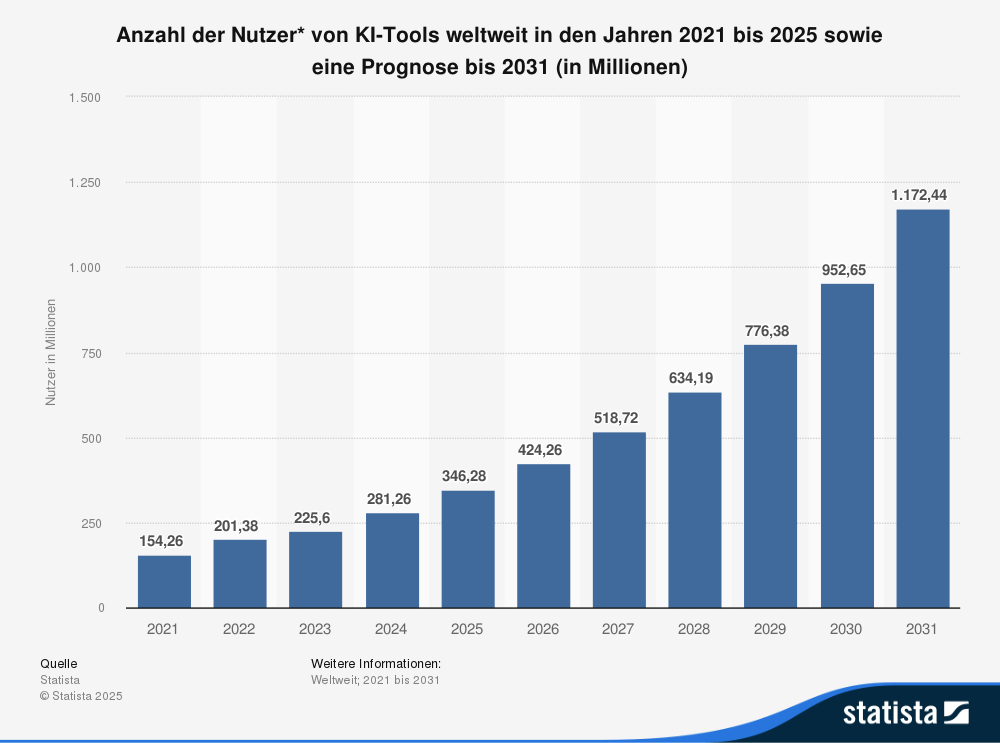
\includegraphics[width=0.7\textwidth]{images/abbildungen/statistic_id1469771_nutzer-von-ki-tools-weltweit-von-2021-bis-2031.png}
    \caption{Nutzer von KI-Tools weltweit von 2021 bis 2031 (Prognose). Quelle: Statista~\cite{statista_ki_nutzer_2031}.}
    \label{fig:ki-nutzerwachstum}
\end{figure}

Generative KI-Tools wirken sich auf sämtliche Phasen des
Softwareentwicklungsprozesses aus, von der Planung über die Implementierung bis
hin zu Test und Deployment, und eröffnen dadurch neue Potenziale für
Effizienzsteigerungen~\cite{minikiewicz_impact_nodate}. Feldexperimente mit
Softwareentwickler:innen belegen, dass sich der Einsatz dieser Werkzeuge
unmittelbar positiv auf Produktivität und Arbeitsweise
auswirkt~\cite{cui_effects_2024}.

Auch komplexere Aufgaben wie Debugging oder die automatische Anpassung von
Datenstrukturen profitieren von KI-Unterstützung, wie insbesondere der
Vergleich zwischen Copilot und Cursor verdeutlicht. Die Literatur verweist
dabei auf Effizienzsteigerungen von bis zu 50\,\% bei
Routinetätigkeiten~\cite{s_future_2024}, was sich mit den im Praxisteil
beobachteten Zeitersparnissen und Produktivitätsgewinnen deckt.

Die Qualität der Automatisierung hängt jedoch stark von der Präzision der
Prompts und der Kontextintegration der eingesetzten Tools ab. Wie die Arbeit
mit Cursor gezeigt hat, ist gerade bei komplexeren Aufgaben ein dialogischer
Ansatz mit Feedback-Loops und manueller Kontrolle weiterhin unverzichtbar.
Dennoch verdeutlichen Forschung und Praxis, dass generative KI einen spürbaren
Effizienzgewinn im Entwicklungsalltag ermöglicht.
Wangoo~\cite{wangoo_artificial_2018} betont darüber hinaus, dass
KI-Technologien nicht nur den Entwicklungsprozess beschleunigen, sondern auch
die Wiederverwendung bestehender Komponenten und das Design von Software
nachhaltig vereinfachen können.